\begin{tikzpicture}[
    arrow/.style={thick,->,shorten >=2pt,shorten <=2pt,>=stealth},
]
    \draw (0,0) rectangle (8,2.5) node at (4,.4) {Aramis}; % ARAMIS
    
    \draw (.5,1) rectangle (2.5,2)  node [pos=.5] {Server}; % GH
    \draw (5.5,1) rectangle (7.5,2) node [pos=.5] {Client}; % GB

    \draw[arrow,green] (-.5,.5) -- (.5,1.25); % Arrow BL
    \draw[arrow,red] (-.5,1.5) -- (.5,1.5); % Arrow ML
    \draw[arrow,red] (-.5,2.5) -- (.5,1.75); % Arrow TL

    \draw[arrow,green] (7.5,1.25) -- (8.5,.5); % Arrow BR
    \draw[arrow,red] (7.5,1.5) -- (8.5,1.5); % Arrow MR
    %\draw[arrow,red] (7.5,1.75) -- (8.5,2.5); % Arrow TR
    
    \draw (3,1) rectangle (5,2) node [pos=.5] {Filter}; % Filters

    \draw (5.5,3) rectangle (7.5,4) node [pos=.5] {Alerts};
    \draw[arrow] (5,2) -- (5.5,3);

    \draw[arrow,blue,very thick] (5,1.25) -- (5.5,1.25); % Arrow SF
    \draw[arrow,blue,very thick] (5,1.5) -- (5.5,1.5); % Arrow SF
    %\draw[arrow,blue,very thick] (5,1.75) -- (5.5,1.75); % Arrow SF

    \draw[arrow,blue,very thick] (2.5,1.25) -- (3,1.25); % Arrow FC
    \draw[arrow,blue,very thick] (2.5,1.5) -- (3,1.5); % Arrow FC
    \draw[arrow,blue,very thick] (2.5,1.75) -- (3,1.75); % Arrow FC

    \draw (3,3) rectangle (5,4) node [pos=.5,align=center] {Efficient\\Rules}; % Rules
    \draw[arrow] (4,3) -- (4,2);

    \draw (3,5) rectangle (5,6) node [pos=.5] {Generation}; % Generator
    \draw[arrow] (4,5) -- (4,4);

    \draw (5.5,5) rectangle (8.1,6) node [pos=.5,align=center] {Domain-specific\\language}; % Rules
    \draw[arrow] (5.5,5.5) -- (5,5.5);

    \draw (0,4.5) rectangle (2,6) node at (.45,5.8) {\tiny Legend:};
    \draw[arrow,blue,very thick] (.2, 5.5) -- (.7,5.5) node [anchor=west] at (.5,5.5) {\tiny Ad-hoc lang.};
    \draw[arrow,red] (.2, 5.12) -- (.7,5.12) node [anchor=west] at (.5,5.12) {\tiny Attack msg.};
    \draw[arrow,green] (.2, 4.75) -- (.7,4.75) node [anchor=west] at (.5,4.75) {\tiny Normal msg.};
    
    \begin{scope}[fill opacity=0.25]
        \draw node  at (10,1.25) {\resizebox{.2\textwidth}{!}{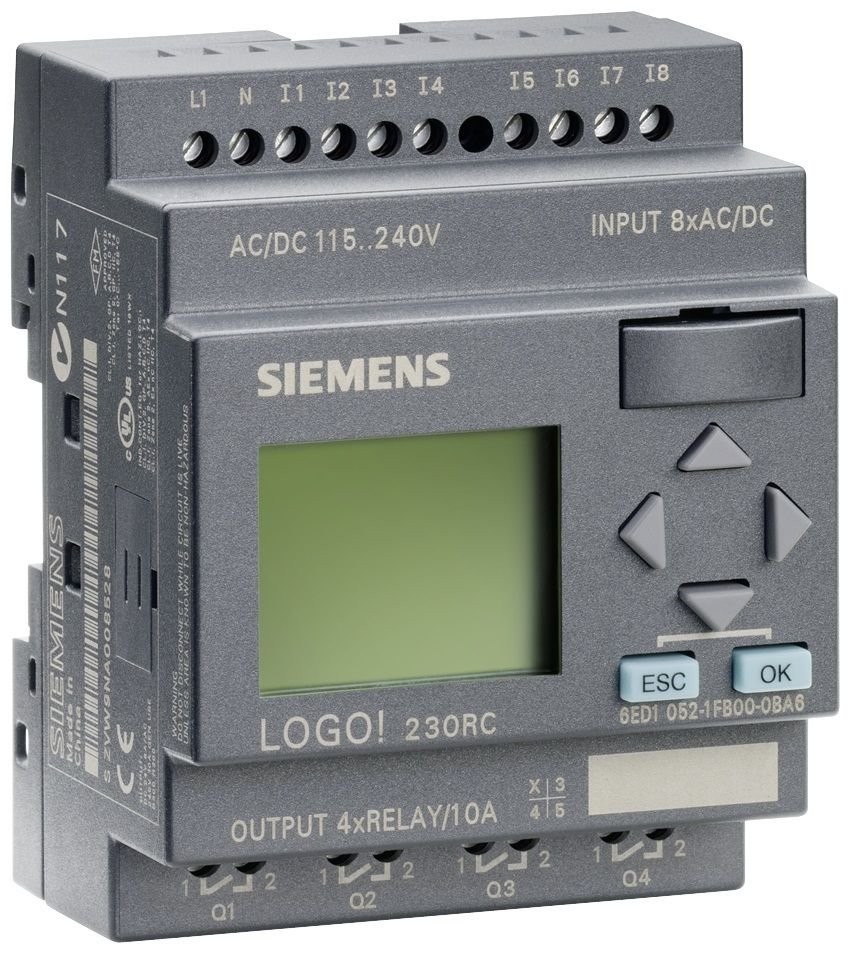
\includegraphics{plc}}};
        \draw node at (-2.8,1.25) {\resizebox{.3\textwidth}{!}{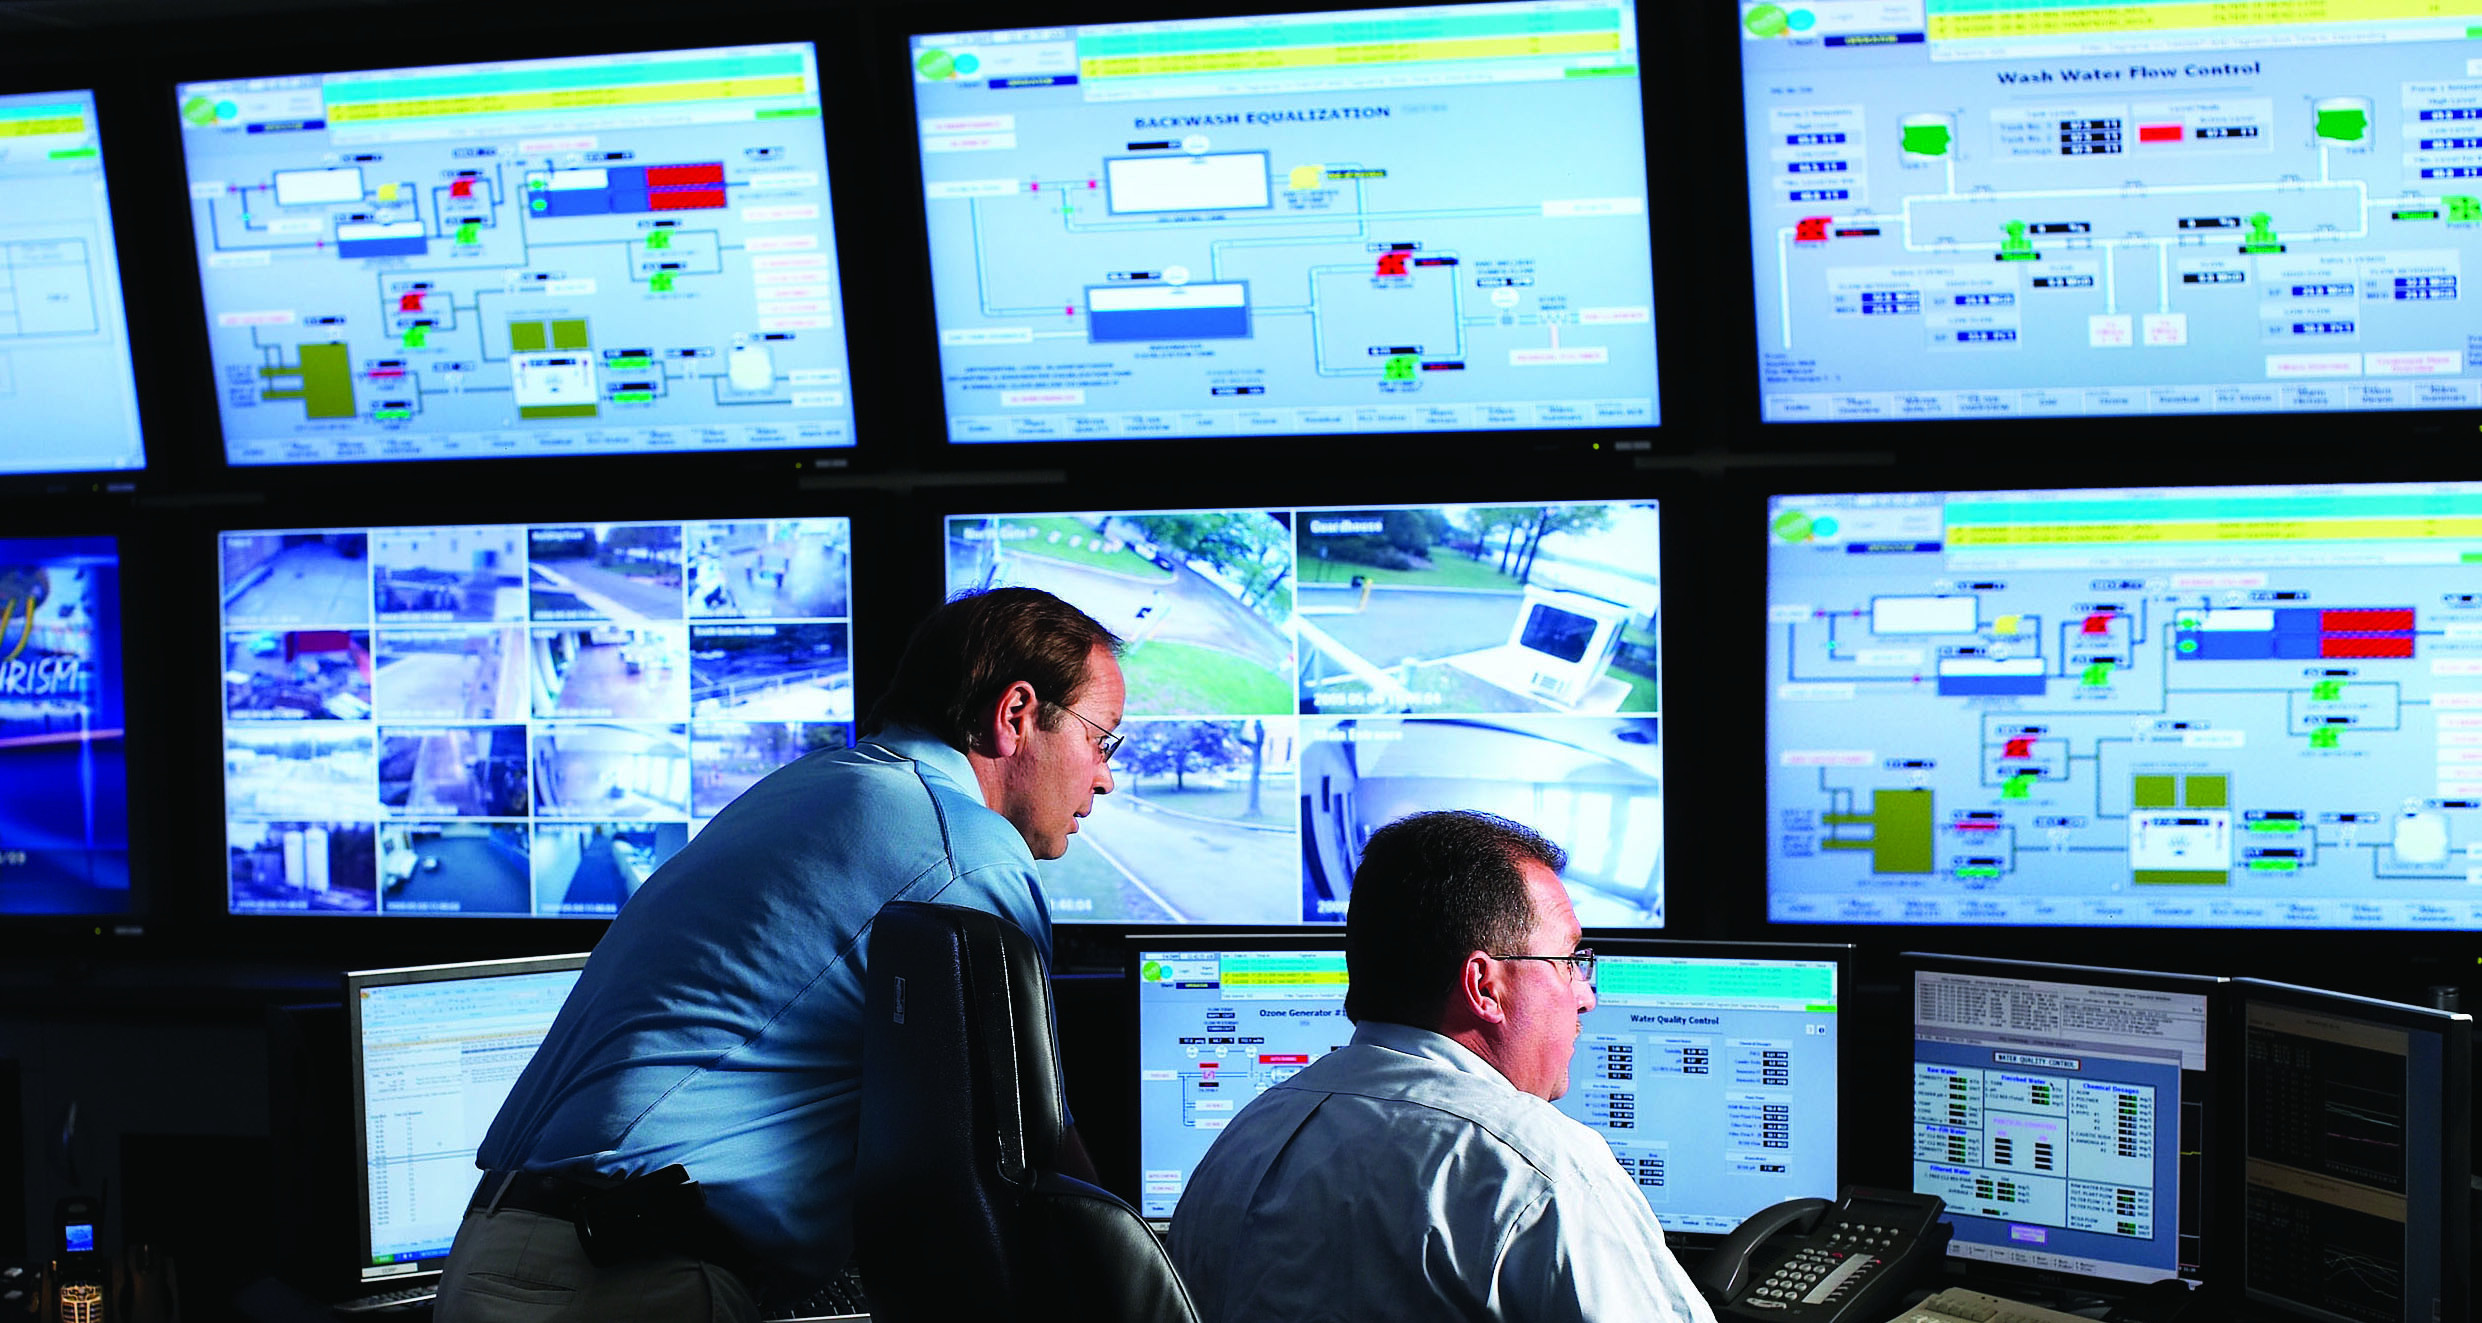
\includegraphics{scada}}};
    \end{scope}
\end{tikzpicture}
